% =====================================================================
%  Self-Healing Task Allocation for Decentralized UAV Swarms under
%  Intermittent Connectivity and Ambiguous Failures
%  IEEEtran journal format -- methodology manuscript (results pending)
%  Compile: pdflatex main && bibtex main && pdflatex main && pdflatex main
%  (or upload the whole latex/ folder to Overleaf)
% =====================================================================
\documentclass[journal]{IEEEtran}

\usepackage[T1]{fontenc}
\usepackage{cite}
\usepackage{amsmath,amssymb}
\usepackage{graphicx}
\usepackage{booktabs}
\usepackage{array}
\usepackage{algorithm}
\usepackage{algpseudocode}
\usepackage{xcolor}
\usepackage{url}
\usepackage[hidelinks]{hyperref}

\newtheorem{assumption}{Assumption}
\newtheorem{proposition}{Proposition}
\newtheorem{lemma}{Lemma}
\newtheorem{definition}{Definition}

% Marker for content that requires experimental data (do NOT remove before results exist)
\newcommand{\pending}[1]{\par\noindent\fcolorbox{red!60!black}{red!5}{\parbox{0.95\columnwidth}{\small\textbf{[RESULTS PENDING]} #1}}\par}
\newcommand{\Rc}{R_{\mathrm{c}}}
\newcommand{\ind}{\mathbf{1}}
\newcommand{\rhomin}{\rho_{\min}}

\begin{document}

\title{Self-Healing Task Allocation for Decentralized UAV Swarms under Intermittent Connectivity and Ambiguous Failures}

\author{[Author Name], [Co-author Name], and [Supervisor Name]%
\thanks{[Author Name] and [Co-author Name] are with the [Department], [University], [City, Country] (e-mail: [author e-mail]).}%
\thanks{[Supervisor Name] is with the [Supervisor Department], [University], [City, Country].}%
\thanks{This manuscript describes a proposed method and a pre-specified evaluation protocol. Sections marked ``Results pending'' will be completed after the experiments are run.}}

\markboth{[Target journal --- to be decided]}{[Author Name] \MakeLowercase{\textit{et al.}}: Self-Healing UAV Task Allocation under Ambiguous Failures}

\maketitle

% ---------------------------------------------------------------------
\begin{abstract}
Decentralized unmanned aerial vehicle (UAV) swarms used for search and rescue lose contact with their members for two very different reasons: drones fly out of communication range, or drones crash. Existing decentralized allocators handle either network partitions or known failures, but not both. In practice the two cases are indistinguishable to the remaining drones: a peer has simply gone silent. Reassigning too early duplicates work and creates conflicting mission state when a live drone returns; reassigning too late leaves the tasks of a crashed drone unserved. This paper proposes a self-healing task allocation architecture that treats this ambiguity explicitly. Each UAV keeps a replica of a mission ledger built from conflict-free replicated data types (CRDTs), which records task completion, ownership claims and evidence of life, and which converges deterministically after network partitions and after wrong failure suspicions. A suspicion estimator combines accrual failure detection with each peer's published plan, and a takeover policy, either a threshold rule or a multi-agent proximal policy optimization (MAPPO) policy trained with centralized training and decentralized execution, decides when a suspected peer's task should be claimed. We formalize the problem, prove that the ledger replicas converge and agree on task ownership, and pre-specify a simulation-based evaluation with eleven scenarios, seven methods including the recent CC-OPI allocator, ten ablations, and a statistical analysis plan. The central quantity studied is the trade-off between task recovery time and duplicated work. Experimental results are pending and are not reported here.
\end{abstract}

\begin{IEEEkeywords}
UAV swarms, decentralized task allocation, intermittent connectivity, failure detection, self-healing systems, conflict-free replicated data types, multi-agent reinforcement learning, search and rescue.
\end{IEEEkeywords}

% =====================================================================
\section{Introduction}
\IEEEPARstart{S}{warms} of small unmanned aerial vehicles (UAVs) can cover a disaster area much faster than a single aircraft, provided that the swarm divides the search area among its members and keeps doing so as conditions change~\cite{R04_chung2018}. In realistic deployments, however, inter-UAV links are short-ranged and lossy, so the swarm repeatedly fragments into groups that cannot communicate~\cite{R21_tegicho2023,R16_oubbati2019}, and individual UAVs fail through battery depletion, collisions or hardware faults.

Decentralized task allocation has responded to each of these problems separately. Market-based algorithms such as the consensus-based bundle algorithm (CBBA) provide conflict-free assignments without a central planner~\cite{R02_choi2009,R03_johnson2011}, and a growing body of work makes them robust to packet loss, limited bandwidth and limited range~\cite{R22_raja2022,R24_tong2026,R25_qian2026,R27_verma2025}. The recent CC-OPI allocator explicitly handles swarms that fragment into ``information islands'' and merges completion records when islands meet~\cite{R66_liu2026}. Separately, replanning methods reassign the tasks of UAVs whose failure is known~\cite{R35_bai2026,R67_giacomossi2026}.

These two lines of work rest on assumptions that cannot hold at the same time. Partition-tolerant allocators assume that UAVs do not crash (CC-OPI states that ``no mid-mission UAV failure are modeled''~\cite{R66_liu2026}); failure-replanning methods assume that failures are known events, typically with global communication~\cite{R67_giacomossi2026}. In a real swarm, a silent UAV may be crashed or merely out of range, and distributed-systems theory shows that no observer can reliably tell the two apart in an asynchronous network~\cite{R05_fischer1985,R06_chandra1996}. Acting on this ambiguity is costly in either direction: a premature takeover duplicates work when the ``failed'' UAV returns, while a delayed takeover leaves the tasks of a crashed UAV unserved. This dilemma between fault correction and fault tolerance has been measured in generic decentralized systems~\cite{R43_nikolic2021}, but not, to our knowledge, in UAV task allocation.

This paper addresses that gap. Our contributions are:
\begin{enumerate}
\item A formal problem statement for decentralized UAV task allocation under \emph{combined} network partitions and crash-stop failures, with ground-truth metrics for duplicated work, false takeovers and censored recovery times (Section~\ref{sec:problem}).
\item A convergent \emph{mission ledger} built from conflict-free replicated data types~\cite{R10_shapiro2011,R11_almeida2024} that extends completion-only merging~\cite{R66_liu2026} to ownership and evidence-of-life state, together with proofs that replicas converge and agree on task ownership (Section~\ref{sec:ledger}).
\item A \emph{plan-aware suspicion estimator} that adapts accrual failure detection~\cite{R07_hayashibara2004} to multi-hop, intermittent evidence and uses each peer's published plan to separate ``silent and expected far away'' from ``silent and expected nearby'' (Section~\ref{sec:suspicion}).
\item A \emph{takeover policy} formulated as a decentralized partially observable Markov decision process and trained with MAPPO~\cite{R62_yu2022} under centralized training and decentralized execution, compared against a tunable threshold rule (Section~\ref{sec:policy}).
\item A pre-specified, reproducible evaluation protocol: eleven scenarios, seven methods including a fair adaptation of CC-OPI, ten ablations, and a statistical analysis plan (Section~\ref{sec:experiments}).
\end{enumerate}

Because the experiments have not yet been run, this manuscript is a methodology paper: it presents the problem, the design, the proofs and the evaluation protocol, and marks every place where experimental data will be required. No experimental result is reported or implied.

The remainder of the paper is organized as follows. Section~\ref{sec:related} reviews related work and states the research gap. Section~\ref{sec:problem} formalizes the problem. Section~\ref{sec:architecture} presents the architecture and its components. Section~\ref{sec:experiments} details the experimental design. Section~\ref{sec:results} defines the results to be reported. Section~\ref{sec:limitations} discusses limitations and future work, and Section~\ref{sec:conclusion} concludes.

% =====================================================================
\section{Related Work and Research Gap}\label{sec:related}

The literature was searched in Crossref, arXiv and the open web using 21 topic queries (2019--2026) supplemented by foundational works; 708 unique records were screened and 72 retained, with metadata verified against Crossref or the publisher. Most evidence is at abstract level; full texts were examined for the closest works~\cite{R66_liu2026,R67_giacomossi2026,R53_goeckner2024,R34_bramblett2023}.

\subsection{Decentralized Task Allocation}
Gerkey and Matari\'c formalized multi-robot task allocation (MRTA) and its taxonomy~\cite{R01_gerkey2004}. CBBA combines market-based bundle construction with a consensus phase and is proven to converge to conflict-free assignments~\cite{R02_choi2009}; its asynchronous variant ACBBA removes synchronous rounds~\cite{R03_johnson2011}. CBBA variants have been applied to search and rescue~\cite{R31_grntved2023} and to large swarms~\cite{R33_rodriguez2025}, and a unified comparison of centralized and distributed allocators, including resilience to UAV failures, is available~\cite{R30_song2025}.

\subsection{Allocation under Imperfect Communication}
Communication-aware CBBA learns to schedule messages under bandwidth limits and collisions~\cite{R22_raja2022}; DTBA-C3 compensates for packet loss and data errors~\cite{R24_tong2026}; LR-PI resolves conflicts under constrained communication~\cite{R23_yan2024}; AC-DMTA suppresses messages that cannot change the assignment under stale information~\cite{R68_zhao2026}; and UCDG-PD uses chance constraints and task-local leases under stochastic links~\cite{R25_qian2026}. Auctions degrade gracefully under lossy auctioneer--bidder links when winner data are re-sent~\cite{R26_otte2020}, and an empirical study compares decentralized allocators under Bernoulli, Gilbert--Elliott and fading channels~\cite{R27_verma2025}. Closest to our setting, CC-OPI interleaves negotiation with execution in a swarm fragmented by a short communication radius, merging completed-task sets by union when islands meet and reporting ``wasted distance'' as the price of robustness~\cite{R66_liu2026}. CC-OPI explicitly excludes mid-mission UAV failures and assumes loss-free links within range.

\subsection{Failure-Triggered Reallocation and Self-Healing}
ES-CBBA escalates the replanning scope after UAV failures~\cite{R35_bai2026}; performance-impact and auction variants reallocate tasks after single or multiple failures~\cite{R36_wang2023,R37_sun2025}; and IRDS reallocates search sectors by reverse auction after injected battery faults, reporting high mission success under workforce loss~\cite{R67_giacomossi2026}. In IRDS the market state is global and failure is ``treated instantaneously as a market event''~\cite{R67_giacomossi2026}. Self-healing work on UAV swarms more often targets formation or topology: recursive grouping restores configuration after individual failures~\cite{R38_pan2025}, and graph-based deep reinforcement learning restores connectivity~\cite{R39_wang2025}. Meeting-based patrolling detects failures at rendezvous points and redistributes responsibilities, but reports cascading failures under some fault conditions~\cite{R41_santhirasegaram2026}.

\subsection{Multi-Agent Reinforcement Learning}
Value-decomposition methods (VDN~\cite{R63_sunehag2018}, QMIX~\cite{R61_rashid2018}) and actor--critic methods (MADDPG~\cite{R64_lowe2017}, MAPPO~\cite{R62_yu2022}) follow the centralized-training, decentralized-execution (CTDE) paradigm, whereas independent learners (IQL~\cite{R75_tan1993}, IPPO~\cite{R76_witt2020}) and networked actor--critic methods~\cite{R77_zhang2018} learn without a centralized component. MARL has been applied to UAV task allocation with communication gating~\cite{R50_xiong2026}, graph embeddings~\cite{R52_ratnabala2026} and asynchronous value decomposition combined with ACBBA~\cite{R51_cao2025}. MAGEC trains a shared graph-neural-network policy with MAPPO for patrolling under agent attrition and message loss~\cite{R53_goeckner2024}; failures are not detected explicitly, and crashed and disconnected agents are not distinguished. MAPPO's robustness to partial agent failure depends strongly on the reward structure~\cite{R57_barta2025}.

\subsection{Distributed-Systems Foundations}
Consensus is impossible in asynchronous systems with even one crash~\cite{R05_fischer1985}; unreliable failure detectors characterize what can be achieved~\cite{R06_chandra1996}; and accrual detectors output a continuous suspicion level rather than a binary verdict~\cite{R07_hayashibara2004}. Gossip-style detectors spread heartbeat counters epidemically~\cite{R74_renesse1998}, and SWIM separates failure detection from membership dissemination~\cite{R08_das2002}. Under partitions, a replicated system must trade consistency for availability~\cite{R09_gilbert2002}. Conflict-free replicated data types (CRDTs) remain available under partition and converge deterministically~\cite{R10_shapiro2011,R11_almeida2024}; delta-state CRDTs reduce synchronization traffic~\cite{R73_almeida2018}, including in opportunistic networks~\cite{R12_guidec2022,R72_guidec2026}. Delay-tolerant networking supplies the store-carry-forward model~\cite{R13_fall2003,R14_spyropoulos2005,R19_xiong2019}.

\subsection{Research Gap}
Table~\ref{tab:related} summarizes the closest works. Communication-robust allocators do not model UAV crashes; failure-reallocation methods assume that failures are known and that communication is reliable; MARL methods that tolerate attrition do not detect failures or reconcile state. No reviewed work (i)~detects failures under partitions, (ii)~replicates ownership and suspicion-related state so that it converges after a wrong suspicion, or (iii)~quantifies the resulting trade-off between recovery time and duplicated work. Because the evidence for several works is at abstract level, this gap statement is bounded by the search described above.

\begin{table}[!t]
\centering
\caption{Closest works. Y = addressed, P = partially, N = not addressed in the material examined, ? = not accessible.}
\label{tab:related}
\footnotesize
\setlength{\tabcolsep}{3pt}
\begin{tabular}{@{}lcccccc@{}}
\toprule
Work & Partitions & Crashes & Detection & Ambiguity & Reconcile & Learning\\
\midrule
CBBA~\cite{R02_choi2009} & P & N & N & N & N & N\\
CA-CBBA~\cite{R22_raja2022} & Y & N & N & N & N & Y\\
UCDG-PD~\cite{R25_qian2026} & Y & N & N & N & P & N\\
CC-OPI~\cite{R66_liu2026} & Y & N & N & N & P & N\\
ES-CBBA~\cite{R35_bai2026} & N & Y & N & N & N & N\\
IRDS~\cite{R67_giacomossi2026} & N & Y & N & N & N & N\\
HMP~\cite{R41_santhirasegaram2026} & Y & Y & Y & ? & ? & N\\
Epistemic~\cite{R34_bramblett2023} & Y & Y & P & P & P & N\\
MAGEC~\cite{R53_goeckner2024} & P & Y & N & N & N & Y\\
TACC~\cite{R50_xiong2026} & Y & N & N & N & N & Y\\
\midrule
This work & Y & Y & Y & Y & Y & Y\\
\bottomrule
\end{tabular}
\end{table}

% =====================================================================
\section{Problem Formulation}\label{sec:problem}

\subsection{Mission and Agents}
The search area is divided into $M$ sectors, each treated as a task $k\in\mathcal{K}=\{1,\dots,M\}$ with centre $\mathbf{q}_k$, service time $s_k>0$ and weight $w_k>0$. The task set is fixed at mission start, and each task requires one UAV (single-task robots, single-robot tasks, time-extended assignment~\cite{R01_gerkey2004}). A task is complete once one UAV has serviced it for $s_k$; any further service is duplicated work.

A homogeneous swarm $\mathcal{N}=\{1,\dots,N\}$ flies at speed $v$ under point-mass kinematics. UAV $i$ has position $\mathbf{p}_i(t)$, energy $e_i(t)$ and true status $\sigma_i(t)\in\{\textsc{alive},\textsc{crashed}\}$; $\sigma_i$ is known only to the simulator and is used solely for evaluation. Energy evolves as
\begin{equation}
e_i(t+\Delta t)=e_i(t)-c_f\,\Delta t\,\ind[\text{active}]-c_m\,n_i^{\mathrm{tx}}(t),
\end{equation}
where $n_i^{\mathrm{tx}}(t)$ is the number of messages transmitted in the step. UAVs know their own position and share a loosely synchronized clock (GNSS time) with bounded skew $\epsilon$.

\subsection{Communication Model}
The communication graph is $\mathcal{G}(t)=(\mathcal{N}_{\mathrm{alive}}(t),\mathcal{E}(t))$ with $(i,j)\in\mathcal{E}(t)$ iff $\|\mathbf{p}_i(t)-\mathbf{p}_j(t)\|\le \Rc$. A message over a link of length $d$ is delivered with probability
\begin{equation}
q(d)=q_0\left(1-(d/\Rc)^{\gamma}\right),\quad d\le \Rc,
\end{equation}
optionally replaced by a two-state Gilbert--Elliott burst-loss channel~\cite{R27_verma2025}. The connected components $\mathcal{C}_1(t),\dots,\mathcal{C}_{c(t)}(t)$ of $\mathcal{G}(t)$ are the partitions. There is no infrastructure; information crosses partitions only when UAVs physically carry it (store-carry-forward~\cite{R13_fall2003}).

\subsection{Failure Model}
Failures are crash-stop: at time $t_j^{c}$ UAV $j$ stops moving and transmitting permanently. Byzantine behaviour and partial degradation are out of scope. A live UAV may also be silent for a long time (out of range, in another partition, or under a radio blackout) and later reconnect. A silent peer is therefore either crashed or disconnected, and the observing UAV cannot know which.

\subsection{Objectives}
The swarm should maximize the weighted mission completion rate while limiting duplicated work. Let $\ind_{ik}(t)$ indicate that UAV $i$ is servicing task $k$ at time $t$, $S_k=\sum_i\int_0^{T_{\max}}\ind_{ik}(t)\,dt$ the total service spent on $k$, and $\mathcal{K}_{\mathrm{done}}$ the tasks completed by $T_{\max}$. The two primary metrics are
\begin{align}
\mathrm{MCR}&=\frac{\sum_{k\in\mathcal{K}_{\mathrm{done}}}w_k}{\sum_{k\in\mathcal{K}}w_k},\label{eq:mcr}\\
\mathrm{DWR}&=\frac{\sum_{k\in\mathcal{K}_{\mathrm{done}}}(S_k-s_k)}{\sum_{k\in\mathcal{K}}s_k}.\label{eq:dwr}
\end{align}
For each task $k$ left unfinished by a UAV $j$ that crashes at $t_j^c$ (an \emph{orphaned} task), the recovery time is $\tau_k^{\mathrm{cl}}=t_k^{\mathrm{claim}}-t_j^c$, where $t_k^{\mathrm{claim}}$ is the first claim on $k$ by another live UAV. Recovery times are right-censored at $T_{\max}$ when no claim occurs.

\subsection{Research Questions and Hypotheses}
\begin{itemize}
\item \textbf{RQ1:} When UAVs cannot tell a crashed peer from a disconnected one, what is the trade-off between recovery time and duplicated work? \textbf{H2:} both vary monotonically with takeover aggressiveness.
\item \textbf{RQ2:} Can a convergent ledger keep mission state consistent across partitions and wrong suspicions, and at what communication cost?
\item \textbf{RQ3:} Does a learned takeover policy improve on a tuned threshold rule? \textbf{H3:} yes under intermittent connectivity, but not under full connectivity.
\item \textbf{RQ4:} How does the complete design compare with centralized, CBBA-based and CC-OPI allocation when partitions and failures co-occur? \textbf{H1:} it completes more of the mission when failures occur and is non-inferior when they do not.
\item \textbf{RQ5:} How do results scale with swarm size, range and failure rate, and does a per-partition coordinator help? \textbf{H4:} the coordinator gives no significant benefit.
\item \textbf{H5:} the plan-aware suspicion term lowers the false-takeover rate at equal recovery time.
\end{itemize}

% =====================================================================
\section{Proposed Architecture}\label{sec:architecture}

\subsection{Design Principles and Overview}
The architecture follows five principles: (i)~every UAV holds a full replica of the mission state and can complete tasks with no peer contact; (ii)~contacts improve coordination but their absence never blocks progress, i.e., availability is preferred over consistency under partition~\cite{R09_gilbert2002}; (iii)~correctness resides in a convergent data structure, not in the network, so learning affects efficiency but never consistency; (iv)~silent peers are \emph{suspected} to a degree, never declared dead~\cite{R07_hayashibara2004}; and (v)~no permanent leader exists. Fig.~\ref{fig:overview} illustrates the setting and Fig.~\ref{fig:components} the onboard components, which are identical on every UAV.

\begin{figure}[!t]
\centering
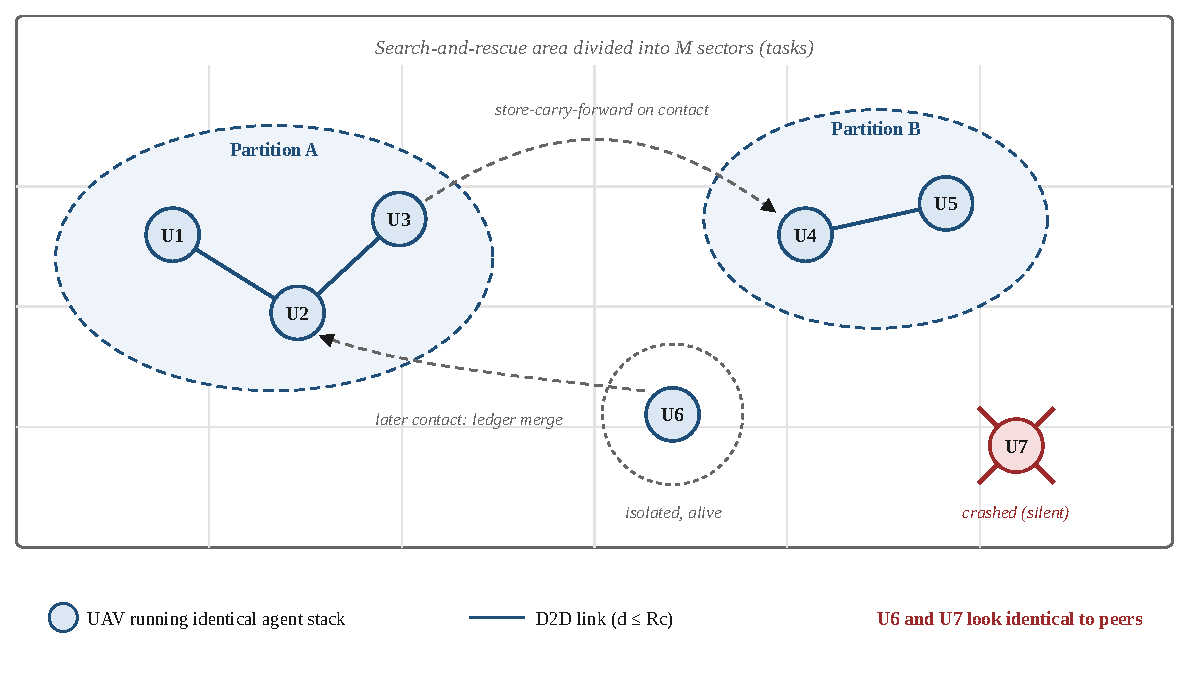
\includegraphics[width=\columnwidth]{figures/fig1_overview.pdf}
\caption{System setting. The swarm forms and loses partitions as UAVs move; information crosses partitions only through store-carry-forward. An isolated live UAV (U6) and a crashed UAV (U7) are indistinguishable to their peers.}
\label{fig:overview}
\end{figure}

\begin{figure}[!t]
\centering
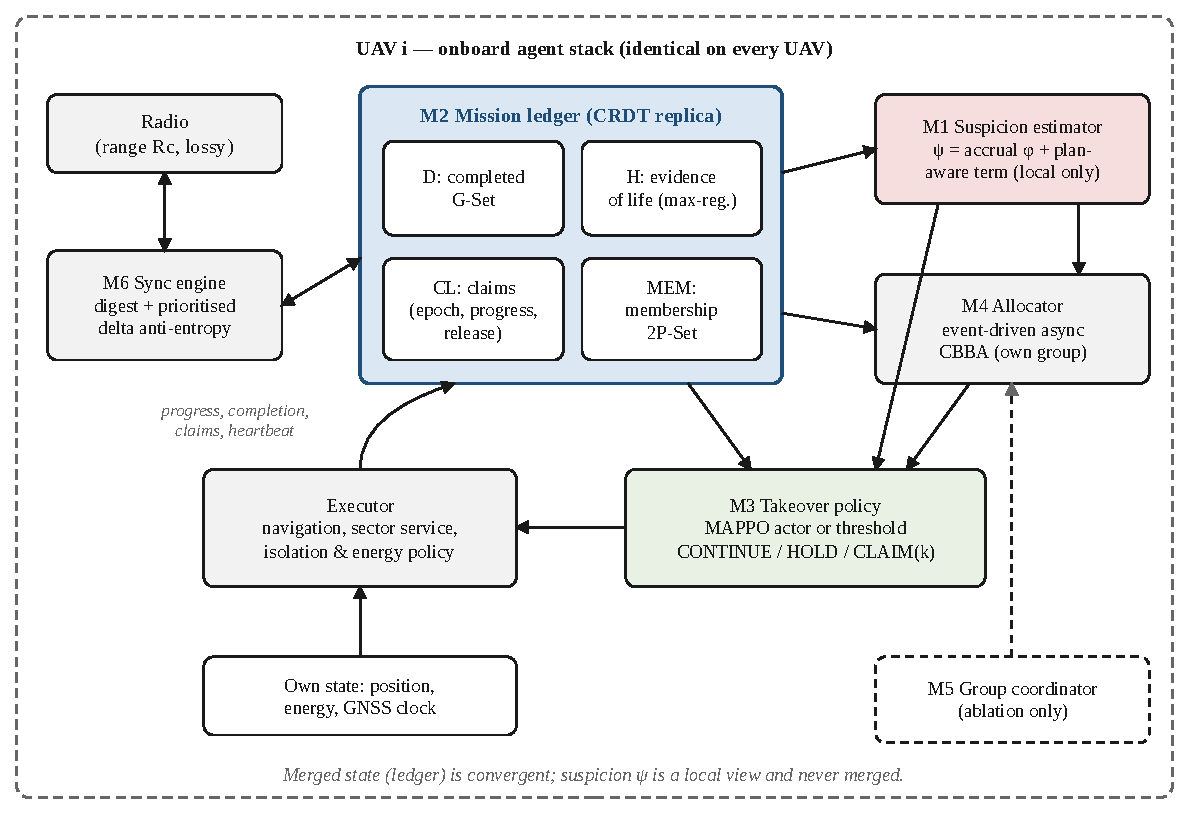
\includegraphics[width=\columnwidth]{figures/fig2_components.pdf}
\caption{Onboard agent stack. The mission ledger (M2) is the only merged state; suspicion (M1) is a local view. The takeover policy (M3) overrides the base allocator (M4) only for tasks whose owner is suspected. The group coordinator (M5) is used only in an ablation.}
\label{fig:components}
\end{figure}

\subsection{Mission Ledger (M2)}\label{sec:ledger}
Each UAV $i$ holds a replica $L_i=(D_i,H_i,\mathit{CL}_i,\mathit{MEM}_i)$. Every component is a join-semilattice whose merge $\sqcup$ is commutative, associative and idempotent, and every local update is an \emph{inflation} (it moves the state upward).

\begin{definition}[Ledger components]
\begin{enumerate}
\item \emph{Completions} $D_i\subseteq\mathcal{K}\times\mathcal{N}\times\mathbb{R}$, a grow-only set merged by union.
\item \emph{Evidence of life} $H_i:\mathcal{N}\to(c,\tau,\mathbf{p},\pi)$: for each UAV $j$ a heartbeat counter $c$, timestamp $\tau$, position $\mathbf{p}$ and published plan $\pi$. Only $j$ increments $c_j$; entries are merged by keeping the larger counter.
\item \emph{Claims} $\mathit{CL}_i:\mathcal{K}\times\mathcal{N}\to(\varepsilon,\rho,r)\in\mathbb{N}\times[0,1]\times\mathbb{N}$: entry $(k,j)$ is written only by UAV $j$ and holds a claim epoch $\varepsilon_{kj}$, progress $\rho_{kj}$ and release epoch $r_{kj}$; the claim is \emph{active} iff $\varepsilon_{kj}>r_{kj}$. Entries are merged component-wise by $\max$.
\item \emph{Membership} $\mathit{MEM}_i=(A_i,R_i)$, a two-phase set; planned departures enter $R_i$, crashes never do.
\end{enumerate}
\end{definition}

Local updates by UAV $j$ on task $k$ are: \emph{claim} $\varepsilon_{kj}\leftarrow 1+\max_\ell\varepsilon_{k\ell}$; \emph{progress} $\rho_{kj}\leftarrow\max(\rho_{kj},\text{new progress})$; \emph{release} $r_{kj}\leftarrow\varepsilon_{kj}$; and \emph{reassert}, which is a claim permitted only when $\rho_{kj}\ge\rhomin$ and $\rho_{kj}$ strictly exceeds the progress of the current owner. The current owner of task $k$ in replica $i$ is
\begin{equation}
o_i(k)=\arg\max_{j:\,\varepsilon_{kj}>r_{kj}}\ (\varepsilon_{kj},\,-j),\label{eq:owner}
\end{equation}
i.e., the active claim with the highest epoch, ties broken by the lowest identifier.

\begin{assumption}[Temporal connectivity]\label{as:tc}
There exists $W<\infty$ such that, for every interval of length $W$, the union of $\mathcal{G}(t)$ over the interval connects all UAVs alive throughout it.
\end{assumption}

\begin{assumption}[Sufficient contacts]\label{as:contact}
Any two UAVs in contact eventually complete a digest-and-delta exchange (possibly over several contacts), since the ledger size is bounded by $O(M N)$ and bandwidth per contact is positive.
\end{assumption}

\begin{lemma}\label{lem:lattice}
The ledger state space, ordered component-wise, is a join-semilattice with join $\sqcup$, and every local update is an inflation.
\end{lemma}
\begin{IEEEproof}
A grow-only set under union and a two-phase set under component-wise union are join-semilattices~\cite{R10_shapiro2011}. For $H$, each entry $j$ is written only by $j$, whose counter strictly increases with every write; hence the map from counter values to tuples is a function, and ``keep the larger counter'' is the join of a totally ordered set lifted to the tuple. For $\mathit{CL}$, each entry is a product of totally ordered sets under component-wise $\max$, which is a join-semilattice; a map of join-semilattices under point-wise join is a join-semilattice, and a finite product of join-semilattices is a join-semilattice. Claim, progress, release and reassert only increase entry components, and heartbeat and completion updates only add or increase, so all updates are inflations.
\end{IEEEproof}

\begin{proposition}[Convergence]\label{prop:sec}
Two replicas that have received the same set of updates are equal, regardless of the order, duplication or delay of delivery. Under Assumptions~\ref{as:tc} and~\ref{as:contact}, every update reaches every UAV that remains alive, so all live replicas converge.
\end{proposition}
\begin{IEEEproof}
By Lemma~\ref{lem:lattice}, each replica's state equals the join of the initial state and the states produced by all updates it has received. Because $\sqcup$ is commutative, associative and idempotent, this join is independent of order and multiplicity, which is the strong-eventual-consistency property of state-based CRDTs~\cite{R10_shapiro2011}. For delivery, consider an update created by UAV $u$ at time $t_0$ and a UAV $x$ alive throughout $[t_0,t_0+W]$. By Assumption~\ref{as:tc} there is a time-respecting sequence of contacts from $u$ to $x$ within the union graph; by Assumption~\ref{as:contact} each contact in the sequence eventually transfers all state that the receiver lacks, including the update, because merged state is retained and re-offered at every subsequent contact. By induction along the sequence, $x$ eventually receives the update.
\end{IEEEproof}

\begin{proposition}[Owner agreement]\label{prop:owner}
The owner function~\eqref{eq:owner} is well defined, and any two replicas with equal $\mathit{CL}$ components assign the same owner to every task.
\end{proposition}
\begin{IEEEproof}
Identifiers are unique, so the pairs $(\varepsilon_{kj},-j)$ are totally ordered and the maximum over a finite non-empty set is unique; if no claim is active, the task has no owner. The function depends only on $\mathit{CL}$, so equal $\mathit{CL}$ implies equal owners.
\end{IEEEproof}

Two remarks delimit these results. First, suspicion values are \emph{not} part of the ledger: they influence which updates a UAV issues, never how updates merge, so Propositions~\ref{prop:sec} and~\ref{prop:owner} hold irrespective of detector quality. Second, replicas may disagree between contacts; the duplicated work caused by such transient disagreement is precisely what the evaluation measures. If Assumption~\ref{as:tc} fails because groups never meet again, no protocol can reconcile them, a limitation shared with CC-OPI~\cite{R66_liu2026}.

\paragraph*{Synchronization} On each new contact, UAVs exchange heartbeats and a compact digest of their ledgers, then send missing deltas~\cite{R73_almeida2018}: first claims and completions that concern tasks of suspected peers, then all remaining deltas, subject to a per-contact bandwidth cap. Lost messages are harmless because the next digest exchange re-offers missing state and duplicate deliveries are absorbed by idempotence.

\subsection{Suspicion Estimator (M1)}\label{sec:suspicion}
For UAV $i$ observing peer $j$, let $\tau_{ij}(t)$ be the timestamp of the freshest evidence of life for $j$ in $H_i$, whether received directly or relayed, and $g_{ij}(t)=t-\tau_{ij}(t)$ the current silence. Following the accrual principle~\cite{R07_hayashibara2004},
\begin{equation}
\phi_{ij}(t)=-\log_{10}\!\left(1-\hat F_j\big(g_{ij}(t)\big)\right),
\end{equation}
where $\hat F_j$ is the estimated distribution of evidence gaps for $j$: a mixture of a prior $F_0$ fitted for the communication setting and the empirical distribution of $j$'s observed gaps, weighted by $n/(n+n_0)$ with $n$ observed gaps. Unlike classical accrual detectors, gaps here are dominated by mobility and partitions rather than by network jitter.

The ledger also holds $j$'s published plan, from which $i$ predicts $j$'s position $\hat{\mathbf{p}}_j(t)$. Let $\eta_{ij}(t)=\ind[\|\mathbf{p}_i(t)-\hat{\mathbf{p}}_j(t)\|\le\beta\Rc]$ indicate that $j$ is expected to be in range, and let $m_{ij}(t)$ be the time during the current silence for which $\eta_{ij}=1$. The combined suspicion is
\begin{equation}
\psi_{ij}(t)=\phi_{ij}(t)+\kappa\,\frac{m_{ij}(t)}{T_{\mathrm{hb}}},\qquad\kappa\ge 0,\label{eq:psi}
\end{equation}
with heartbeat period $T_{\mathrm{hb}}$. Silence while expected far away increases suspicion slowly; silence while expected nearby increases it quickly. Hypothesis H5 tests whether this term improves discrimination between crashed and disconnected peers; $\kappa=0$ is an ablation.

\subsection{Base Allocator (M4)}
Within each connected group, UAVs run an event-driven asynchronous CBBA~\cite{R02_choi2009,R03_johnson2011}. The path score is $S_i(\pi_i)=\sum_{k\in\pi_i}w_k\lambda_d^{\tau_{ik}(\pi_i)}$ with time discount $\lambda_d\in(0,1)$, and bundles are built from tasks that are not complete and not owned by an unsuspected peer. Re-bundling is triggered by topology changes, completions, new claims or changes in task availability, in the spirit of CC-OPI's event-driven replanning~\cite{R66_liu2026}. Allocation outcomes are written as ledger claims, so allocation and takeover share a single ownership record. Tasks owned by suspected peers are not bid on automatically; they are passed to the takeover policy.

\subsection{Takeover Policy (M3)}\label{sec:policy}
A task $k$ is an \emph{orphan candidate} for UAV $i$ if it is incomplete and its owner $o_i(k)$ has $\psi_{i,o_i(k)}\ge\Phi_{\mathrm{open}}$. The takeover decision is formulated as a decentralized partially observable Markov decision process $\langle\mathcal{N},\mathcal{S},\{\mathcal{A}_i\},P,R,\{\Omega_i\},O,\gamma_d\rangle$:
\begin{itemize}
\item \emph{Observation} $o_i$: own position, energy and bundle length; features of the $K$ highest-ranked orphan candidates (relative position, $w_k$, $s_k$, owner suspicion $\psi$, silence $g$, owner's last progress, number of active claimants); and up to $L$ neighbours. Sets are encoded by attention pooling~\cite{R78_iqbal2019}, making the input independent of $N$ and $M$.
\item \emph{Actions} $\mathcal{A}_i=\{\textsc{continue},\textsc{hold},\textsc{claim}(1),\dots,\textsc{claim}(K)\}$ with masking of invalid options.
\item \emph{Decision epochs}: event-triggered by suspicion level crossings, new orphans or task completion, with a periodic fallback; rewards between epochs are accumulated.
\item \emph{Team reward}
\begin{equation}
r_t=\sum_{k\in\mathcal{K}_t^{\mathrm{new}}}\big(w_k-\lambda\,\mathrm{Dup}_k\big)-\lambda\sum_{k}\mathrm{post}_k(t)-\mu\sum_i\Delta e_i(t),\label{eq:reward}
\end{equation}
where $\mathcal{K}_t^{\mathrm{new}}$ are tasks completed at $t$, $\mathrm{Dup}_k$ is the service spent on $k$ by UAVs other than the completer (charged at completion), and $\mathrm{post}_k(t)$ is service at $t$ on an already completed task. Both terms are causal.
\end{itemize}

The policy is trained with MAPPO~\cite{R62_yu2022} using a shared actor for all UAVs and a centralized critic $V_\psi(s)$ that, during training only, observes the true status of every UAV. This privileged critic is discarded at execution, so deployment remains fully decentralized. To obtain the whole trade-off curve from one training run, $\lambda$ is sampled per episode and supplied as an input to actor and critic. We chose MAPPO over QMIX and VDN because value-decomposition mixers either assume a fixed team size or cannot represent ``exactly one UAV should take over''; IPPO~\cite{R76_witt2020} serves as an ablation to test the value of the centralized critic. As a non-learned baseline, the \emph{threshold rule} claims the nearest orphan whose owner has $\psi\ge\Phi$, and sweeping $\Phi$ traces its trade-off curve.

\subsection{Failure Recovery, Isolation and Optional Coordinator}
Fig.~\ref{fig:recovery} shows the recovery workflow. If the suspected peer has crashed, the claimant completes the task and self-healing is achieved. If the peer was alive, merging resolves the conflict deterministically: the returning UAV reasserts if its progress is at least $\rhomin$ and exceeds the claimant's progress, and otherwise yields. Fig.~\ref{fig:example} gives a concrete example.

\begin{figure}[!t]
\centering
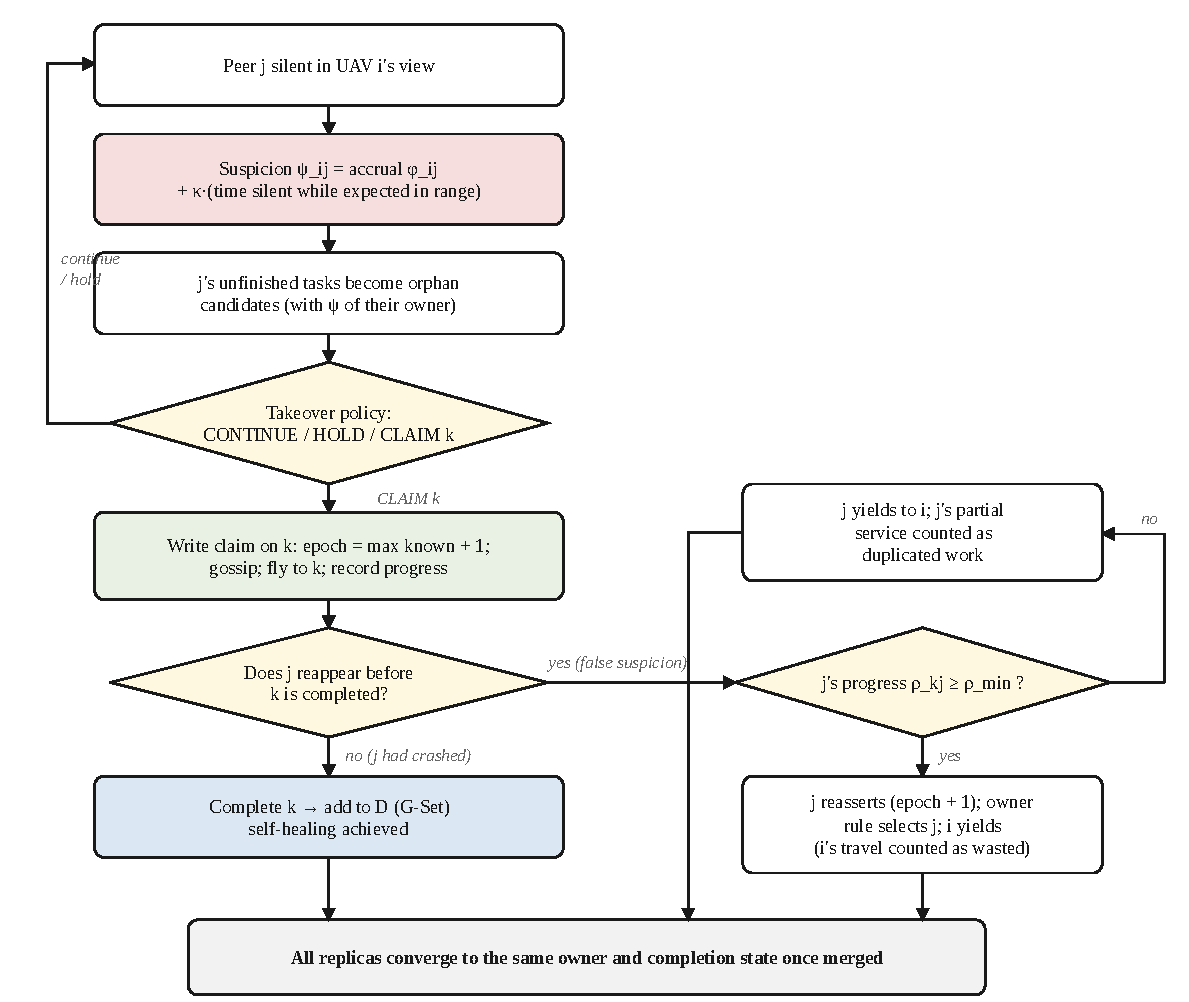
\includegraphics[width=\columnwidth]{figures/fig3_recovery.pdf}
\caption{Failure-recovery workflow. Both error types are measured: wasted or duplicated work after a false suspicion, and delayed claiming when the peer has truly crashed.}
\label{fig:recovery}
\end{figure}

\begin{figure}[!t]
\centering
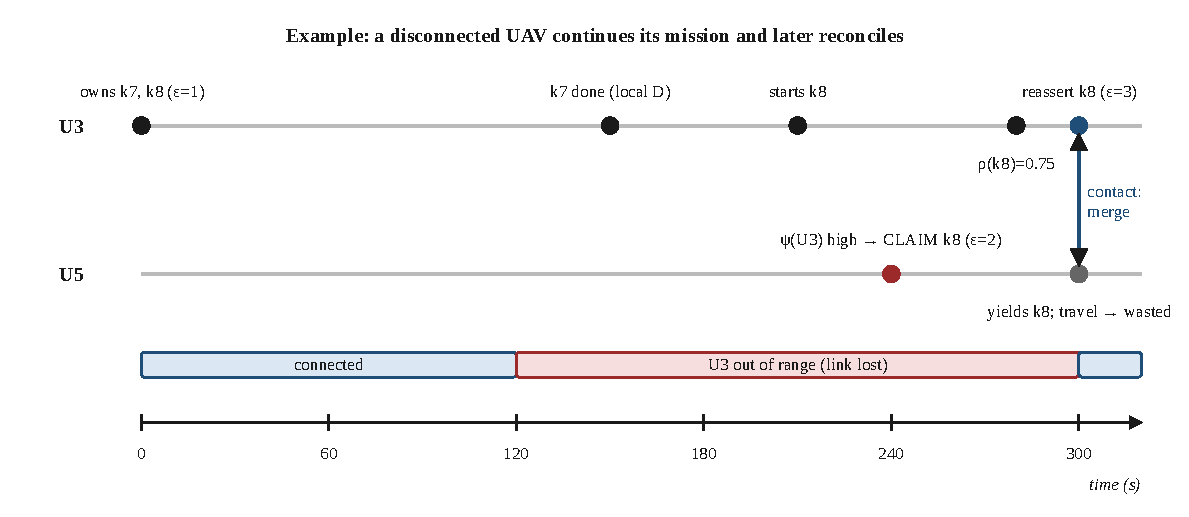
\includegraphics[width=\columnwidth]{figures/fig4_example.pdf}
\caption{Illustrative example (not an experimental result). U3 loses contact, completes k7 alone, and is suspected by U5, which claims k8 with a higher epoch. When contact resumes, U3 has progressed further on k8 and reasserts; U5 yields and its travel is counted as wasted.}
\label{fig:example}
\end{figure}

A UAV without contact follows an isolation policy: it finishes its own bundle, then claims the nearest task that is open in its own replica, periodically diverts toward the last known position of the largest group to attempt a rendezvous, and returns to base when its remaining energy covers only the return flight plus a margin. For the leader ablation (H4), each connected group derives a coordinator deterministically from the ledger (the unsuspected member with the most energy, ties broken by identifier) holding a renewable lease. Unlike Raft~\cite{R65_ongaro2014}, a minority partition still obtains a coordinator; concurrent coordinators are resolved by lease epoch when groups merge, and ownership is always decided by~\eqref{eq:owner}.

\subsection{Algorithms}
Algorithms~\ref{alg:loop} and~\ref{alg:sync} summarize the per-UAV loop and the contact exchange.

\begin{algorithm}[!t]
\caption{Per-UAV control loop (UAV $i$, every $\Delta t$)}\label{alg:loop}
\begin{algorithmic}[1]
\State advance executor (move or service current task $k$)
\State update $\rho_{ki}$; \textbf{if} $k$ completed \textbf{then} $D_i\gets D_i\cup\{(k,i,t)\}$
\If{$t \bmod T_{\mathrm{hb}}=0$} increment $c_i$; publish $(c_i,t,\mathbf{p}_i,\pi_i)$ in $H_i$ \EndIf
\For{each neighbour $j$ in range} \Call{SyncExchange}{$i,j$} \EndFor
\State update $\psi_{ij}$ for all $j\neq i$ using~\eqref{eq:psi}
\If{topology, ledger or suspicion event} re-bundle with asynchronous CBBA over open tasks in current group \EndIf
\If{decision epoch}
  \State $a\gets$ policy$(o_i)$ \Comment{MAPPO actor or threshold rule}
  \If{$a=\textsc{claim}(k)$} $\varepsilon_{ki}\gets 1+\max_\ell\varepsilon_{k\ell}$ \EndIf
\EndIf
\If{$o_i(k)\neq i$ for current task $k$}
  \If{$\rho_{ki}\ge\rhomin$ and $\rho_{ki}>\rho_{k,o_i(k)}$} reassert \Else{} $r_{ki}\gets\varepsilon_{ki}$ \EndIf
\EndIf
\State apply isolation and energy policy
\end{algorithmic}
\end{algorithm}

\begin{algorithm}[!t]
\caption{\textsc{SyncExchange}$(i,j)$}\label{alg:sync}
\begin{algorithmic}[1]
\State exchange heartbeats and ledger digests (version vectors)
\State $\Delta_{\mathrm{prio}}\gets$ missing claims/completions for tasks of suspected peers
\State $\Delta_{\mathrm{rest}}\gets$ all other missing deltas
\State send $\Delta_{\mathrm{prio}}$ then $\Delta_{\mathrm{rest}}$ within bandwidth cap; defer remainder
\State on receipt of $\Delta$: $L_i\gets L_i\sqcup\Delta$ \Comment{order-free, idempotent}
\State raise events for changed completion, owner or availability
\end{algorithmic}
\end{algorithm}

% =====================================================================
\section{Experimental Design}\label{sec:experiments}

The protocol below is fixed before any experiment is run; later changes will be logged with date and reason.

\subsection{Simulation Environment}
A discrete-time Python simulator implements kinematics, energy, the channel models and failure injection, with a PettingZoo-compatible interface for training. MAPPO is implemented in PyTorch. Correctness checks include property-based tests of the CRDT laws (random update sequences delivered in random orders with duplicates must yield identical replicas), owner agreement after full merge, hand-verified micro-scenarios for every metric, and determinism under fixed seeds. Table~\ref{tab:params} lists the default parameters, all of which are modelling assumptions rather than measured values.

\begin{table}[!t]
\centering
\caption{Default simulation parameters (assumptions)}
\label{tab:params}
\footnotesize
\begin{tabular}{@{}lll@{}}
\toprule
Parameter & Default & Sweep\\
\midrule
Area & $2000\times1500$\,m & ---\\
UAVs $N$; tasks $M$ & 10; 30 & $N\in\{6,10,16,24,32\}$, $M=3N$\\
Service time $s_k$ & $\mathcal{U}(150,250)$\,s & ---\\
Speed $v$; endurance & 10\,m/s; 1800\,s & ---\\
Range $\Rc$ & 400\,m & $\{200,400,800,\infty\}$\\
Delivery $q(d)$ & $q_0=0.95$, $\gamma=2$ & Gilbert--Elliott variant\\
Heartbeat $T_{\mathrm{hb}}$ & 1\,s & ---\\
Crash fraction $f$ & 0 & $\{0,0.1,0.2,0.3\}$\\
Clock skew $\epsilon$ & 0\,s & $\{0.5,2\}$\,s\\
Horizon $T_{\max}$; step $\Delta t$ & 1800\,s; 0.5\,s & ---\\
$\rhomin$; $K$; $\beta$ & 0.5; 5; 0.8 & pilot-tuned\\
\bottomrule
\end{tabular}
\end{table}

\subsection{Scenarios}
Table~\ref{tab:scenarios} defines the scenarios. A \emph{blackout} silences a live UAV's radio for $T_s$ seconds while it continues to fly and work; this creates the ambiguous case with known ground truth. For each random seed, every method faces the identical world, failure schedule and channel realization (common random numbers).

\begin{table}[!t]
\centering
\caption{Scenario matrix}
\label{tab:scenarios}
\footnotesize
\begin{tabular}{@{}p{0.6cm}p{7.4cm}@{}}
\toprule
ID & Definition\\
\midrule
S1 & Normal: $\Rc=\infty$, no loss, no failures\\
S2 & Interruption: 20\% of UAVs suffer one blackout, $T_s\in\{60,180,400\}$\,s; no crashes\\
S3 & Partition: forced split for $T_p\in\{120,300,600\}$\,s\\
S4 & Single crash at a random time\\
S5 & Leader/critical failure: coordinator (or UAV with most unfinished tasks) crashes\\
S6 & Multiple failures: $f=0.3$, staggered crashes\\
S7 & Expansion: start with 7 UAVs, 3 join at 300\,s\\
S8 & Reduction: 3 UAVs announce departure at 300\,s\\
S9 & Combined: S3 ($T_p=300$\,s) + $f=0.2$ (one crash on minority side) + blackouts on 10\%\\
S10 & Ambiguity stress: 2 crashes and 2 blackouts at matched times\\
S11 & S9 with clock skew $\epsilon\in\{0.5,2\}$\,s\\
\bottomrule
\end{tabular}
\end{table}

\subsection{Methods, Baselines and Ablations}
The compared methods are: B0, a centralized oracle with global communication and instant failure knowledge (upper bound); B1, greedy nearest-task (lower bound); B2, CBBA/ACBBA with timeout-based reassignment~\cite{R02_choi2009,R03_johnson2011}; B3a, CC-OPI re-implemented as published~\cite{R66_liu2026}; B3b, CC-OPI with the same timeout rule as B2, a fair adaptation to the failure setting; P1, the proposed design with the threshold rule; and P2, the proposed design with MAPPO. The CC-OPI re-implementation must reproduce its published completion rate in its own setting (within five percentage points) before use. Ablations remove or replace one component at a time: completion-only merge (A1), binary timeout instead of accrual suspicion (A2), $\kappa=0$ (A3), epoch-first and progress-first owner rules (A4, A5), first-in-first-out instead of prioritized exchange (A6), full-state instead of delta synchronization (A7), per-group coordinator (A8), IPPO instead of MAPPO (A9), and MAPPO without the privileged critic (A10). Each method's key parameter is tuned on separate validation seeds with an equal budget of eight grid points.

MAPPO is trained on $N\in\{6,10,16\}$, $\Rc\in\{200,400,800\}$, crash fractions in $[0,0.3]$ and random blackouts and partitions, with five independent training seeds, and evaluated on unseen seeds and on $N\in\{24,32\}$.

\subsection{Metrics}
Beyond MCR~\eqref{eq:mcr} and DWR~\eqref{eq:dwr}, the evaluation reports the following.
\begin{itemize}
\item \emph{Time and allocation efficiency}: completion time $T_{\mathrm{mc}}$; coverage $\mathrm{AUC}=T_{\max}^{-1}\int_0^{T_{\max}}\mathrm{MCR}(t)\,dt$; and allocation efficiency relative to the oracle's discounted score.
\item \emph{Waste and recovery}: wasted-distance ratio~\cite{R66_liu2026}; claim latency $\tau^{\mathrm{cl}}$ and service-resumption time; and the fraction of orphaned tasks never recovered.
\item \emph{Error rates}: false-takeover rate $\mathrm{FTR}=\#\{\text{claims while previous owner alive}\}/\#\{\text{claims}\}$ and its cost.
\item \emph{Detector quality}: the area under the ROC curve (AUROC) of $\psi$ over silent pairs labelled crashed or alive (S10).
\item \emph{Ledger consistency}: owner divergence $\mathrm{Div}(t)$, the fraction of co-located replica pairs and tasks with differing owners; and time to consistency after partition merges.
\item \emph{Network}: packet delivery ratio; update dissemination latency (mean and 95th percentile, censored); mean component count; and pairwise connectivity.
\item \emph{Cost and scalability}: messages and bytes per completed task; energy per completed task; autonomy during isolation (tasks completed while isolated relative to tasks owned); leader recovery time (A8); and decision computation time versus $N$.
\end{itemize}
The trade-off between median $\tau^{\mathrm{cl}}$ and DWR is summarized by the normalized hypervolume of each method's front.

\subsection{Statistical Analysis Plan}
Each configuration is evaluated on 30 seeds (validation and training seeds are disjoint). Paired comparisons use the Wilcoxon signed-rank test~\cite{R81_wilcoxon1945} with Holm correction within each hypothesis family~\cite{R80_holm1979}; effect sizes are matched-pairs rank-biserial correlations with 95\% bootstrap confidence intervals. Recovery times are analysed with Kaplan--Meier estimators~\cite{R79_kaplan1958}, log-rank tests and restricted mean survival time, because unrecovered tasks are censored. MARL results are aggregated across training seeds with interquartile means and stratified bootstrap intervals~\cite{R82_agarwal2021}. Table~\ref{tab:hyp} lists the decision rule for each hypothesis; H1 includes a non-inferiority margin of two percentage points in failure-free scenarios. Thirty paired seeds give approximately 80\% power for a standardized paired effect of about 0.55; if pilot variance is higher, the seed count will be increased before the main runs.

\begin{table}[!t]
\centering
\caption{Hypotheses and decision rules}
\label{tab:hyp}
\footnotesize
\begin{tabular}{@{}p{0.55cm}p{1.35cm}p{6.0cm}@{}}
\toprule
H & Data & Supported if\\
\midrule
H1 & S4, S6, S9; S1, S3 & P1/P2 $>$ B2 and B3b on MCR (Holm-adjusted $p<0.05$) and lower CI of (P $-$ B3a) $>-2$\,pp in S1/S3\\
H2 & S2, S9, S10 & Spearman correlation of $\Phi$ with $\tau^{\mathrm{cl}}$ positive and with DWR negative (CIs exclude 0)\\
H3 & S9 sweep & HV(P2) $-$ HV(P1) CI $>0$ at $\Rc\le400$\,m and includes 0 at $\Rc=\infty$\\
H4 & S5, S9 & MCR equivalence of A8 and P1 within $\pm2$\,pp (TOST)\\
H5 & S10, S9 & AUROC($\kappa>0$) $>$ AUROC($\kappa=0$) and lower FTR at matched median $\tau^{\mathrm{cl}}$\\
\bottomrule
\end{tabular}
\end{table}

% =====================================================================
\section{Results and Discussion}\label{sec:results}

\pending{No experiment has been run. This section specifies what will be reported; it contains no data.}

\subsection{Planned Results}
Table~\ref{tab:results} is the template for the main results. Figures to be produced are: (i)~recovery-time versus duplicated-work fronts for B2, B3b, P1 and P2 on S9; (ii)~Kaplan--Meier recovery curves on S6 and S9; (iii)~completion rate and overhead versus $N$; (iv)~hypervolume difference between P2 and P1 versus $\Rc$; (v)~ROC curves of $\psi$ with and without the plan-aware term; (vi)~owner divergence around partition merges for P1 and A1; and (vii)~MAPPO training curves across training seeds.

\begin{table*}[!t]
\centering
\caption{Template for main results on S9 and S1 (median [95\% CI]); all cells pending}
\label{tab:results}
\footnotesize
\begin{tabular}{@{}lcccccccc@{}}
\toprule
Method & MCR (S9) & $T_{\mathrm{mc}}$ (S9) & DWR (S9) & $\tau^{\mathrm{cl}}$ (S9) & UF (S9) & FTR (S9) & kB/task (S9) & MCR (S1)\\
\midrule
B0 Oracle & --- & --- & --- & --- & --- & --- & --- & ---\\
B1 Greedy & --- & --- & --- & --- & --- & --- & --- & ---\\
B2 CBBA+timeout & --- & --- & --- & --- & --- & --- & --- & ---\\
B3a CC-OPI & --- & --- & --- & --- & --- & --- & --- & ---\\
B3b CC-OPI+timeout & --- & --- & --- & --- & --- & --- & --- & ---\\
P1 Proposed (threshold) & --- & --- & --- & --- & --- & --- & --- & ---\\
P2 Proposed (MAPPO) & --- & --- & --- & --- & --- & --- & --- & ---\\
\bottomrule
\end{tabular}
\end{table*}

\subsection{Interpretation Plan}
Each hypothesis can fail, and failures will be reported. If H3 is not supported, the learned policy offers no advantage over a tuned threshold, which would indicate that the trade-off is governed mainly by the suspicion signal rather than by the decision rule; the ledger and detector contributions would remain. If H5 is not supported, the plan-aware term will be removed from the recommended design. If the proposed design is not non-inferior to CC-OPI in failure-free scenarios, the overhead of ownership and evidence replication will be quantified and discussed as the cost of failure awareness.

\pending{Discussion of observed trade-offs, comparison with CC-OPI and IRDS behaviour reported in~\cite{R66_liu2026,R67_giacomossi2026}, and practical guidance for choosing takeover aggressiveness.}

% =====================================================================
\section{Limitations and Future Work}\label{sec:limitations}
The study is simulation-based and abstracts flight dynamics, collision avoidance and wind; the channel model uses disk connectivity with distance-dependent and bursty loss but no medium-access contention, a limitation shared with CC-OPI~\cite{R66_liu2026}. Only crash-stop failures are modelled; Byzantine and degraded behaviour are excluded. The task set is fixed and tasks are atomic and single-UAV; dynamic task arrival, heterogeneous UAVs and multi-UAV tasks are natural extensions. Convergence relies on temporal connectivity (Assumption~\ref{as:tc}) and loosely synchronized clocks, whose sensitivity is tested in S11. The literature review used Crossref, arXiv and web search and examined several works only at abstract level; confirmatory searches in IEEE Xplore and Scopus and full-text checks of~\cite{R41_santhirasegaram2026,R42_chatterjee2024} remain to be done. Future work includes validation of the channel model in ns-3, software-in-the-loop flight simulation, hardware experiments, and extending the plan-aware detector with learned motion models.

% =====================================================================
\section{Conclusion}\label{sec:conclusion}
This paper identified a gap between partition-tolerant and failure-aware task allocation for UAV swarms: in practice a silent UAV may be crashed or merely disconnected, and acting on that ambiguity trades recovery time against duplicated work. We proposed a self-healing architecture in which a CRDT-based mission ledger guarantees convergence of completion and ownership state after partitions and wrong suspicions, a plan-aware accrual detector grades suspicion, and a threshold or MAPPO takeover policy decides when to act. We proved convergence and owner agreement under stated assumptions and pre-specified a reproducible evaluation with baselines, ablations and statistical tests. The experimental evaluation is the next step; its results will determine which of the stated hypotheses hold.

% =====================================================================
\section*{Acknowledgment}
[To be completed by the authors.]

\bibliographystyle{IEEEtran}
\bibliography{references}

\end{document}
